\documentclass[a4paper,openright,12pt]{book}
%\documentclass[b5paper,openright,11pt]{book}
\usepackage[utf8]{inputenc}
\usepackage{graphicx,color}
\usepackage[dvipsnames]{xcolor}
\usepackage{amsfonts}
\usepackage{amsmath}
\usepackage{amssymb}
\usepackage{verbatim}
\usepackage{cite} 
\usepackage{fancyhdr}
\usepackage{epigraph}
\usepackage{caption}
\usepackage{psfrag}
\usepackage{hyperref}
\usepackage{pdfpages}
\captionsetup[figure]{font=footnotesize,labelfont=footnotesize}
\graphicspath{{../figures/}}
%To use a kind of times new roman font style
\usepackage{mathptmx}
\usepackage{newtxtext,newtxmath}
\usepackage[titletoc]{appendix}
%To modify the space before title of each chapter
%\usepackage{titlesec}
%\titleformat{\chapter}[display]   
%{\normalfont\huge\bf}{\chaptertitlename\ \thechapter}{20pt}{\Huge}   
%\titlespacing*{\chapter}{0pt}{-10pt}{40pt}
%Modificar encabezado y pie de página.
\pagestyle{fancy}
\fancypagestyle{chapters}{%
\fancyhead{}
\fancyhead[LE,RO]{\thepage}
\fancyhead[RE]{Nanoscale hydrodynamics near solids}
\fancyhead[LO]{{\color{Gray}CHAPTER \thechapter } \leftmark }
\fancyfoot{}
\renewcommand{\headrulewidth}{0.5pt}
}
%\fancyfoot[LE,RO]{\thepage}
%\fancyfoot[LO,CE]{Chapter \thechapter}
%\fancyfoot[CO,RE]{Author Name}
\fancypagestyle{noHeader}{%
\fancyhead{}
\renewcommand{\headrulewidth}{0pt}
}

%New commands
\renewcommand{\thefootnote}{\roman{footnote}}
\newcommand{\esc}{\!\cdot\!}
\newcommand{\Note}[1]{{\bf \color{red}#1}}    % comments and notes
\newcommand{\Pep}[1]{{\color{blue}#1}}     % del libro de Pep
\newcommand{\Pendiente}[1]{{\color{green}#1}} % Revisar
\newcommand{\Tirar}[1]{{\color{Magenta}#1}}   % tirar
\newcommand{\llangle}{\left\langle}
\newcommand{\rrangle}{\right\rangle}
\newcommand{\llg}{\left\lgroup}
\newcommand{\rlg}{\right\rgroup}
\newcommand{\bra}{\llbracket}
\newcommand{\ket}{\rrbracket}
\newcommand{\cc}{\!\parallel\!}
\newcommand{\GK}[2]{\langle#1 \cc #2\rangle}
\newcommand{\GKrest}[2]{\langle#1 \cc #2\rangle^0}

%% Some details about the dissertation.
%\title{Nanoscale hydrodynamics near solids}
%\author{Diego Duque Zumajo}
%\advisor{Dr. Pep Español Garrigós}
%
%
%% ... about the degree.
%\degree{Programa de doctorado en Ciencias}
%
%\field{Sciences}
%\degreeyear{2019}
%\degreemonth{March}
%\department{Department of Fundamental Physics\\Faculty of Sciences}
%
%% ... about the candidate's previous degrees.
%\pdOneName{Master Universitario en Combustibles y Energías para el futuro}
%\pdOneSchool{Universidad Nacional de Educación a Distancia}
%\pdOneYear{2015}
%
%\newcommand{\firstpage}{
%  \thispagestyle{empty}
%
%\begin{flushright}
%  
\includegraphics[height=64pt]{logoED}
%\end{flushright}
%\vspace*\{\fill}
%
%\vspace{5pt}
%\begin{center}
%\Huge \textsc{Tesis Doctoral} \normalsize \\
%
%\vspace{20pt}
%
%\Huge {\@degreeyear} \normalsize \\
%\vspace{5pt} 
%\today
%\vspace{40pt}
%
%\textsc{\Huge \textcolor{midgrey}{\thetitle} \normalsize} \\
%
%\vspace{20pt}
%
%\textsc{\Large \theauthor \normalsize} \\
%
%\vspace{20pt}
%
%\textsc{\large \@pdOneName \normalsize} \\
%
%\vspace{50pt}
%
%\tikz[remember picture,overlay] \node[opacity=0.1,inner sep=0pt] at (current page.center){\includegraphics[width=0.6\paperwidth,height=0.6\paperwidth]{escudoUNED}};
%
%\vspace{15pt}
%
%\textsc{\Large \textcolor{midgrey}{\@degree} \normalsize} \\
%\vspace{20pt}
%\textsc{\large Director: \@advisor\normalsize} \\
%\end{center}
%\vspace*{\fill}
%}
%\renewcommand{\maketitle}{
%\firstpage
%}
%
%\newcommand{\copyrightpage}{
%\newpage
%\thispagestyle{empty}
%\begin{flushright}
%
\includegraphics[height=48pt]{logoED}
%\end\{flushright}
%\vspace*{\fill}
%
%{\scshape \noindent Doctoral dissertation at the Department of
%Fundamental Physics in the Faculty of Science, UNED.}
%\vspace{0.5em}
%
%\noindent \begin{tabular}{lp{10cm}}
%\noindent {\bf  Title:}  & Nanoscale hydrodynamics near solids\\
%\noindent {\bf Author:} & Diego Duque Zumajo
%, M. Sc. in Energies and Fuels for the future. \\
%\noindent {\bf Director:} & Dr. Pep Español Garrigós.
%\\
%\end{tabular}
%\vspace*{\fill}
%
%{\scshape \noindent Tesis doctoral presentada en el Departamento
%de Física Fundamental de la Universidad Nacional de Educación a Distancia.}
%\vspace{0.5em}
%
%\noindent \begin{tabular}{lp{10cm}}
%
%\noindent {\bf Título:} &  Hidrodinámica cerca de paredes. \\
%\noindent {\bf Autor:} & Diego Duque Zumajo, Máster Universitario en Energías y Combustibles para el futuro. \\
%\noindent {\bf Director:} & Dr. Pep Español Garrigós.\\
%\end{tabular}
%\vspace*{\fill}
%\noindent\textcolor{SchoolColor}{\rule{\textwidth}{2pt}}\par
%% \noindent\rule{\textwidth}{0.1em}
%\begin{center}
%
\includegraphics{UNED/by-nc-sa.eps} \\
%
%\scshape \noindent \small \copyright \ \small \theauthor, 
%\@degreeyear \\
%This work is licensed under a Creative Commons
%Attribution-NonCommercial-ShareAlike 4.0 International \\
%(CC BY-NC-SA 4.0) License.
%\end{center}
%\newpage
%\rm
%}
%
%\begin{document}
%%\maketitle
%%\copyrightpage


\begin{document}
\begin{titlepage}
\begin{center}
\begin{Huge}
\textsc{Nanoscale hydrodynamics \\ near solids}
\end{Huge}
\end{center}
\end{titlepage}


\newpage
\pagestyle{noHeader}
Info requerida por la escuela de doctorado
\thispagestyle{empty} % para que no se numere esta pagina

%%\pagestyle{noHeader}
%%\chapter*{}
%%\pagenumbering{Roman} % para comenzar la numeracion de paginas en numeros romanos
%%\begin{flushright}
%%blablabla
%%\end{flushright}
\newpage
\pagenumbering{Roman} % para comenzar la numeracion de paginas en numeros romanos

\tableofcontents % indice de contenidos

\chapter*{Acknowledgments} % si no queremos que añada la palabra "Capitulo"
%\addcontentsline{toc}{chapter}{Agradecimientos} % si queremos que aparezca en el índice
\markboth{Acknowledgments}{Acknowledgments} % encabezado 
blablabla

\chapter*{Abstract} % si no queremos que añada la palabra "Capitulo"
%\addcontentsline{toc}{section}{Abstract} % si queremos que aparezca en el índice
\markboth{Abstract}{Abstract} % encabezado
blablabla

\chapter*{Resumen} % si no queremos que añada la palabra "Capitulo"
%\addcontentsline{toc}{section}{Resumen} % si queremos que aparezca en el índice
\markboth{Resumen}{Resumen} % encabezado
blablabla

\chapter*{Notation, conventions and quotes}

Functions of microstates z in phase space are denoted with a hat as in $\hat{A}(z)$. We follow this convention except for probability densities, as in $\rho_t(z)$. Operators are denoted with ${\cal CALIGRAPHIC}$ symbols. Vectors and matrices are denoted with {\bf boldfaces}.
%We use a number of superscripts for matrices. $M^T$ is the transpose of $M$ , $M^S = (M+M^T )/2$ is the symmetric part of the matrix M while $M^A = (M-M^T )/2$ is the antisymmetric part. 

\Tirar{
We follow Einstein summation convention in which, for example the product of two matrices in components is written as
\begin{align}
    (AB)_{\mu\nu} = A_{\mu\nu}B_{\nu\sigma}=\sum_{\nu}A_{\mu\nu}B_{\nu\sigma} \nonumber
\end{align}
The derivative of a composite function is expressed as
\begin{align}
    \frac{\partial}{\partial x}F(g(x))=\frac{\partial F}{\partial g}(g(x))\frac{\partial g}{\partial x}(x) \nonumber
\end{align}
}

The quotes in the beginning of each chapter are taken from books I read over the time I have spent working in this dissertation, the last four years. I have respected the language in which the writter wrote the book. 


%\pagenumbering{arabic}
%\setcounter{chapter}{-1}

\setcounter{chapter}{-1}
\chapter{Introduction}\label{Chap:Intro}
\pagenumbering{arabic}
%\setcounter{chapter}{-1}
\pagestyle{chapters}  %define page style for the chapters
\markboth{Introduction}{Introduction}
\epigraph{\textit{Falta cita.}}{Título \\ AUTOR}

\Pendiente{\begin{itemize}
    \item Hay veces en que defino el hamiltoniano como $\hat{H}(z)$ y otras como $\hat{H}_N(z)$ 
\end{itemize}}

\Note{Viene de la introducción del paper I}
There  is great  interest  in  the behaviour  of  fluids  in the  nano
\cite{Bocquet2010} and micro  \cite{Lauga2005,Bocquet2011} scales.  At
nanoscales  the structure  of the  fluid starts  playing an  important
role.  The standard  description of structured fluids is  based on the
(classic) Density Functional Theory \cite{Evans1979}, with the density
functional   capturing  all   the  relevant   information  about   the
\textit{equilibrium} state  of the fluid.   In recent years  there has
been a  great interest in  obtaining \textit{dynamic} versions  of the
Density Functional Theory  (DDFT) that would allow one  to discuss not
only equilibrium structured fluids and its correlations but also their
dynamic  behaviour \cite{Lowen2003,Evans2016}.   Since the  pioneering
work by Marconi and Tarazona  \cite{Marconi2000}, which was based on a
Smoluchowski description  for colloidal particles,  several approaches
have been considered  for the formulation of dynamic  versions of DFT,
ranging from  kinetic theory  \cite{Guo2006}, to  projection operators
\cite{Espanol2009d},  and variational  approaches \cite{Schmidt2013}.
Most    existing    works     deal    with    colloidal    suspensions
\cite{Goddard2012,Evans2016}. However, there exist  still a gap in the
treatment  of the dynamics of \textit{simple}  fluids \textit{near  solids} at  scales
where  the  structure  of  the  fluid  is  relevant.   Note  that  the
interaction of  the solid with  the fluid  is the responsible  for the
structuring  of the  density  field near  a wall  (which  is a  purely
reversible and equilibrium effect) but also for irreversible processes
that can be understood, at macroscales, as boundary conditions for the
fluid \cite{Bedeaux1976,Bocquet1994}.

In  Ref.   \cite{Espanol2009d}  we   have  formulated  DDFT  based  on
projection operator  techniques, where the  density field is  the only
relevant variable.  This is appropriate for colloidal systems that are
suspended in  a solvent acting as  a thermal bath.  In  that case, the
density field should  be rather understood as  the concentration field
which,  being  conserved, is  expected  to  be  a slow  variable.   By
selecting  the density  field as  the only  relevant variable,  we are
implicitly assuming that the density  evolves in time scales which are
much larger than  the time scales corresponding to  other variables in
the system.  In contrast to  colloidal systems, simple fluids have the
momentum density and energy density  as conserved variables, and these
variables may  evolve in  comparable time scales  as the  density.  We
have  recently extended  DDFT  to {\em  non-isothermal} situations  by
including the energy density  field \cite{Anero2013}.  Recent attempts
in that direction  have also been taken  by Schmidt \cite{Schmidt2011}
and Wittkowski et al.  \cite{Wittkowski2012}.  The resulting theory is
valid  for \textit{quiescent}  fluids  or solids  in which  convective
motion is not present.  In the  present work, we consider the mass and
momentum density fields of a fluid, allowing to address moving fluids,
but  we do  not  consider energy  transfer. This  is,  we assume  that
momentum transfer is  not affected by energy fluxes. This  is the case
in isothermal  processes or even under  slight temperature differences
whenever the adiabatic coefficient is  close to one, as corresponds to
a practically  incompressible liquid  like water at  room temperature.
The  natural thermodynamic  potential is  the free  energy functional,
instead   of   an   entropy   functional   as   introduced   in   Ref.
\cite{Anero2013}.  In future work we will address the energy transport
at nanoscales.
\Note{Fin de la introducción del paper I}







In Chapter \ref{Chap:NESM} we introduce the Non-Equilibrium Statistical Mechanics


We will see that one important  objective within Non-Equilibrium  Statistical Mechanics
is the derivation of the governing dynamics of a set of coarse-grained
(CG) variables that describe the system at a mesoscopic or macroscopic
level of description  by starting from the microscopic  laws of motion
of the constituent atoms and  molecules of the system \cite{Kubo1991}.
In this quest, the projection  operator technique, as described in the
textbook by Grabert \cite{Grabert1982}, has  proved to be an extremely
useful  tool.   As  discussed   there,  there  are  essentially  three
different  types of  projection operator  theories, associated  to the
names  of   Mori  \cite{Mori1965},  Zwanzig   \cite{Zwanzig1961},  and
Kawasaki  and Gunton  \cite{Kawasaki1973},  with  increasing order  of
generality \cite{Grabert1982}. The Kawasaki-Gunton projection operator
allows one to  obtain non-linear closed equations for  the averages of
the coarse-grained variables. The Zwanzig  projector is a special case
of  the Kawasaki-Gunton  projector  when the  selected variables  are,
instead of  the CG variables themselves,  the \textit{distribution} of
the  CG variables.  This results  into  a governing  equation for  the
probability distribution of CG  variables.  Finally, Mori projector is
obtained    from    Zwanzig     projector    in    near    equilibrium
situations\cite{Grabert1982,Kauzlaric2011a}.   The  resulting  dynamic
equations in  Mori theory are  linear and  allow one to  obtain simple
equations not only for the averages  of the CG variables, but also for
their correlation functions.

The projection operator technique  provides closed and exact equations
for the  evolution of the averages or probabilities  of the CG variables  with only one
assumption about  the initial  distribution of microstates,  which are
assumed   to  be   distributed   with  a   maximum  entropy   ensemble
\cite{Grabert1982}. The exact equations of  motion of the CG variables
contain a reversible  term which is local in time  and an irreversible
integro-differential term describing memory  about the past history of
the CG variables.  The memory  kernel is defined in microscopic terms,
but is completely untractable, as  it involves the so called projected
dynamics which  is different, in  general, from the  usual Hamiltonian
dynamics of the system.

When the  selected CG  variables are  such that  they display  a clear
separation  of time  scales in  its dynamics  then it  is possible  to
resort  to the  Markovian  approximation in  which  the memory  kernel
becomes proportional to  a delta function in time.   Such a separation
of  time scales  happens, in  general, when  the evolution  of the  CG
variables  is the  result of  many minuscule  and fast  contributions.
Under  the Markovian  approximation, the  resulting governing  dynamic
equations    are   non-linear    differential   equations    for   the
non-equilibrium averages  of the  CG variables in  the Kawasaki-Gunton
projector or stochastic  differential equations (SDE) in  the Mori and
Zwanzig projectors.   Within the  Markovian approximation  one obtains
the  transport coefficients  governing  the irreversible  part of  the
dynamics in terms of the time  integral of the time derivatives of the
CG  variables.   These formulae  for  transport  coefficients are  the
celebrated Green-Kubo formulae \cite{Green1952,Kubo1957}.


Chapter \ref{Chap:Theory} corresponds to the published paper \ref{Camargo20018}.\\
Chapter \ref{Chap:Planar} corresonds to the publised paper \ref{}.\\
Chapter \ref{Chap:PBC} corresponds to the published paper \ref{} and \ref{}.\\
Chapter \ref{Chap:Walls} corresponds to the publised paper \ref{} and \ref{}.\\
Chapter \ref{Chap:Slip} corresponds to the publised paper \ref{}.\\


%-----------------------------------------------------------------
%CHAPTER 1
%-----------------------------------------------------------------
\chapter{Non-Equilibrium \\ Statistical Mechanics}
\label{Chap:NESM}
\markboth{Non-Equilibrium Statistical Mechanics}{}
\epigraph{\textit{Le temps est une invention du mouvement. Celui qui ne bouge pas ne voit pas le temps passer.}}{Métaphysique des tubes \\ AMÉLIE NOTHOMB}

\section{Introduction}
It was in the nineteen century when the Statistical Mechanics (SM) was born mainly because of the work of Ludwing Boltzmann and Josiah Willard Gibbs. The goal was to reconcile the Thermodynamics with the microscopic laws. 

Thermodynamics was well-established because it draws its concepts from experiments while the attemps to understand it from the Newton's laws collided with problems such as the imposibility of taking into account the interactions between all the particles of a thermodynamic system, the highly nontrivial of theses interactions, the huge number of degrees of freedom or the Loschmidt's paradox\footnote{The second law of thermodynamics estabishes that the entropy of an isolated system increases with time. This can be understood as a time direction imposed by the increasing of the entropy. Furthermore, Newton's laws are reversible. According to Josef Loschmidt this apparently conflict could be the responsible of the imposibility to derive the laws of the thermodynamics from the microscopic laws.}. 
To avoid these problems physicist realized that the macro properties of a thermodynamic system does not strongly depend on the exact dynamics of every particle, but more on the averages that eventually polish the details of the behaviour of the particles. 
Thus, the link between the microscopic and macroscopic theory of matter can be stated appling statistical techniques to the microscopical mechanics laws. 
The connection is posible to the notion of \textit{ensemble}, which is a collection of imaginary systems with a set of common macroscopic properties.  

In this way we may define SM as a theoretical framework which allows to study the macro-properties of a many-body system from the dynamics of its microcopic constituents.
Therefore, we may roughly say that SM acts as a bridge between two levels of description: microscopic level governed by the Newton's laws of motion and the macroscopic level where which is measure with experiments.
A beautiful but rough example about how SM works can be found in the latter book of Dean Rickles, {\it Philosophy of Physics} \cite{Rickles2016}.
He imagines a large musical ensemble playing in concert.
The ``global'' sound produced by the musicians is analogue to the thermodynamic variables obtained from the colisions between the particles in the system. 
The music can me analized from two levels: the global level, where the harmony and the musical form take an important role, and the individual level, in which we focus in what the musicians are playing to produce the global sound. ``In this zooming in and out'', in words of Rickles, ``from the whole system to its parts, that characterizes the relationship between statistical mechanics and thermodynamics: you won't see harmonies in a single bassoon; likewise, you won't see pressure or temperature in an individual molecule.''

The equilibrium theory of SM provides an interpretation for the equilibrium thermodynamic systems from a molecular point of view.
However, most of the phenomena present in the Nature are in non-equilibrium situations. 
Einstein \cite{Einstein1905}, Onsager \cite{Onsager1931} and Kirkwood \cite{Kirkwood1946} made important contributions to Non-Equilibrium Statistical Mechanics (NESM) years before Green \cite{Green1952, Green1954}, in the fifties, formulated it as we know nowadays. 
It was in the 60's when Zwanzig \cite{Zwanzig1961} and Mori \cite{Mori1965} reformulated the theory using the technique of the projection operators \cite{Grabert1982}. 


In this chapter, we review fundamental concepts of SM such as phase space, phase point and phase trajectory.
We introduce from Classical Mechanics (CM) the Hamilton's equations to describe the time evolution of a phase point in the phase space. 
Because of the non-linearity of these equations we write them in the language of the linear operators, where the Liouville operator $i{\rm L}$ plays an important role in the dynamics of the microstates. 
This techniques allows us to obtain the Hamilton's equations as first order differential equations. 
With these equations the trajectory of a phase point is deterministic, but we can not avoid the fact that we have no access to the position and momenta of all particles of the system. 
We introduce the concept of probability density in order to take into account our lack of knowledge of the initial condition. 
Therefore, the evolution of a phase point in the phase space converts into a stochastic process where the evolution of the probability density  is governed by the Liouville equation.
We review the Lioville theorem that tell us that the evolution of a bunch of phase point inside a volume must be conserved (i.e. the volumen must be the same but not the shape). 

In this chapter, we review the Theory of Coarse-Graining (ToCG) which allows one to describe the dynamics with variables that capture the essential information of the system and evolve much more slowy than the neglected ones. 
%These selected coarse variables evolve much more slowy than the neglected variables. 

Finally, we introduce the time-dependent projection operator technique to derive the evolution equation of the selected variables. This technique is an aproximation of the time dependent ensemble, solution of the Liouville equation, with a relevant ensemble plus a correction responsible of the irreversible behaviour. This relevant ensemble is obtained maximizing the entropy functional of Gibbs-Jaynes. 


\section{Hamilton's equations and the evolution of the microstates}
Consider a system consisting of $N$ particles of mass $m$ in a volume $V$. 
In CM the positions of the particles ${\bf q}^N\equiv ({\bf q}_1,\dots,{\bf q}_N)^T$ and their 3N momenta ${\bf p}^N\equiv ({\bf p}_1,\dots,{\bf p}_N)^T$ specify the state of the system at any time. 
The collection of the positions and momenta of the particles defines the microscopic state of the system, $z=(q,p)^T$, which is a {\it phase point} in the {\it phase space} $\Gamma$ of 6N dimensions. 
The notation emphasized that $z$ is a column vector, where $T$ is the transpose. 
Therefore, the time evolution of a phase point $z_t$ is called the {\it phase trajectory} and it is determined by the Hamilton's equations of motion

\begin{equation}
    \dot{{\bf q}}_i = \frac{\partial \hat{H}}{\partial {\bf p}_i}, \dot{{\bf p}}_i = -\frac{\partial \hat{H}}{\partial {\bf q}_i}
  \label{HamiltonEqs}
\end{equation}

Typically the Hamiltonian has the form
\begin{align}
    \hat{H}(z) = \sum_{i=1}^{N}\frac{{\bf p}_i^2}{2m}+\hat{U}({\bf q}_1,\dots,{\bf q}_N)+\sum_{i=1}^{N}\Phi({\bf q}_i),
\end{align}

where the first sum is the kinetic energy of the system, the potential of interaction
between particles is $\hat{U}({\bf q}_1,\dots,{\bf q}_N)$ and $\Phi({\bf r})$ is a time-independent external potential. 

Note that the the phase trajectories can not pass through the same point of the phase space because the evolution of the phase point is subject to 6N initial conditions. 
Thus, if two trajectories in phase space cross is because they started at the same phase point.  

Hamilton's equations can be written in compact form as
\begin{align}
  \dot{z}_t = J\cdot\frac{\partial\hat{H}}{\partial{z}}(z_t)\equiv \hat{v}(z_t),
  \label{compactHamiltonEqs}
\end{align}

where we have defined the Hamiltonian vector field $\hat{v}(z_t)$ and $J$ is the symplectic matrix\footnote{J is an orthogonal matriz, $J^TJ=1\to J^T = J^{-1}$, and its square is the minus the identity matrix $J^2=-1$} with the form
$$
\begin{pmatrix} 
  0 & +1_{3N} \\
  -1_{3N} & 0 
\end{pmatrix},
$$
where $1_{3N}$ is the identity matrix of dimension $3N \times 3N$.

Hamilton's equation (\ref{compactHamiltonEqs}) indicates that the trajectory of $z_t$ in phase space is an integral curve of the velocity field. Therefore, if we follow the indications given by the velocity field we can figure out which microstate will be the next one. 


\subsection{Linear Hamilton's equations}
In the last section we have presented Hamilton's equations as a {\it set of non-linear ordinary differential equations}. However, in the language of linear operators we may obtain linear equations that are amenable of theoretical treatment. 

By analogy with Quantum Mechanics (QM) we consider all functions $\hat{B}(z)$ in phase space as a Hilbert vector space. 
Each function $\hat{B}(z)$ is a vector in the infinite-dimensional Hilbert space vector. 
As well as the state vector in QM, $|\Psi\rangle$, each function (vector) $\hat{B}$ has the dimension of all the possible microstates in which the system might be. 
The identity function in phase space is denoted as $\hat{z}$. It takes any microstate $z$ into $\hat{z}(z)=z$. 
We carefuly distinguish the argument $z$, which is a point in the phase space, from the vector of the Hilbert space $\hat{z}$, which represents the identity function.

The {\it Liouville operator} $i{\cal L}$ is an important operator in the dynamics of the microstatates. It has the following explicit form 
\begin{equation}
    i{\cal L} = -
    \sum_i\left[\frac{\partial \hat{H}}{\partial {\bf q}_i}
\frac{\partial    }{\partial {\bf p}_i}-
\frac{\partial \hat{H}}{\partial {\bf p}_i}
\frac{\partial }{\partial {\bf q}_i}\right]
\label{iL}
\end{equation}
In order to give a more compact form of the action of the Liouville operator on a phase function we introduce the Poisson bracket
\begin{align}
  \{\hat{A},\hat{B}\}\equiv\left(\frac{\partial\hat{A}}{\partial z}\right)^T\cdot J\cdot\frac{\partial\hat{B}}{\partial z}= 
  \sum_i\left[\frac{\partial \hat{A}}{\partial {\bf q}_i}
    \frac{\partial \hat{B}}{\partial {\bf p}_i}-          
    \frac{\partial \hat{A}}{\partial {\bf p}_i}
  \frac{\partial\hat{B} }{\partial {\bf q}_i}\right]
    \label{PoissonBracket}
\end{align}
%\begin{align}
%  \{\hat{A},\hat{B}\}\equiv\left(\frac{\partial\hat{A}}{\partial z}\right)^T\cdot J\cdot\frac{\partial\hat{B}}{\partial z}= 
%  \sum_i\left[\frac{\partial \hat{A}}{\partial {\bf q}_i}
%    \frac{\partial \hat{B}}{\partial {\bf p}_i}-          
%    \frac{\partial \hat{A}}{\partial {\bf p}_i}
%  \frac{\partial\hat{B} }{\partial {\bf q}_i}\right]
%    \label{PoissonBracket}
%\end{align}
Therefore, taking an arbitrary phase function $\hat{B}(z)$ the Liouville operator acts on it in this way
%\begin{align}
%  i{\cal L}\hat{B}=-\left(\frac{\partial\hat{H}}{\partial z}\right)^T\cdot J\cdot\frac{\partial\hat{B}}{\partial z}
%  =\hat{v}^T\cdot\frac{\partial\hat{B}}{\partial z}
%  = \frac{\partial^T}{\partial z}\cdot\left(\hat{H}\hat{B}\right) 
%  = -\{\hat{H},\hat{B}\}
%  \label{iLB}
%\end{align}
\begin{equation}
  i{\cal L}\hat{B} 
%  =-    \sum_i\left[\frac{\partial \hat{H}}{\partial {\bf q}_i}
%      \frac{\partial\hat{B}}{\partial {\bf p}_i}-
%\frac{\partial \hat{H}}{\partial {\bf p}_i}
%\frac{\partial\hat{B} }{\partial {\bf q}_i}\right]
%=-\left(\frac{\partial\hat{H}}{\partial z}\right)^T\cdot J\cdot\frac{\partial\hat{B}}{\partial z}
  = -\{\hat{H},\hat{B}\}
\label{iL}
\end{equation}

Where we have introduce the {\it Poisson bracket} to give a more compact form of the action of the Liouville operator on a phase function. 

%In order to give a more compact form of the action of the Liouville operator on a phase function we have introduced the Poisson bracket
%\begin{align}
%  \{\hat{A},\hat{B}\}\equiv\left(\frac{\partial\hat{A}}{\partial z}\right)^T\cdot J\cdot\frac{\partial\hat{B}}{\partial z}= 
%  \sum_i\left[\frac{\partial \hat{A}}{\partial {\bf q}_i}
%    \frac{\partial \hat{B}}{\partial {\bf p}_i}-          
%    \frac{\partial \hat{A}}{\partial {\bf p}_i}
%  \frac{\partial\hat{B} }{\partial {\bf q}_i}\right]
%    \label{PoissonBracket}
%\end{align}

The action of the Liouville operator on the identity function $\hat{z}$ is
\begin{align}
  i{\cal L} \hat{z} = \hat{v}
  \label{iLz}
\end{align}

Therefore, in the language of the Liouville operator we can transform a complicated nonlinear function $\hat{v}$ into the action of a linear operator $i{\cal L}$ on the identity function $z$.

With the Eq. (\ref{iLz}) the Hamilton's equations (\ref{compactHamiltonEqs}) can be written in terms of the Liouville operator as
\begin{align}
  \frac{d}{dt}z_t=i{\cal L}\hat{z}(z_t)
  \label{Devzt}
\end{align}

In order to obtain an expresion for $z_t$ we consider a Taylor expansion of the trajectory $z_t$ around $t=0$, this is
\begin{align}
    z_t=z_0+\frac{dz_t}{dt}(0)t+\frac{1}{2!}\frac{d^2z_t}{dt^2}(0)t^2+\cdots
    \label{ztExp}
\end{align}
From (\ref{Devzt}) we have the first order derivative. All the high order time derivatives are given by
\begin{align}
    &\frac{d^2z_t}{dt^2} = \frac{d}{dt}i{\cal L}\hat{z}(z_t)
    =\hat{v}^T(z_t)\cdot\frac{\partial i{\cal L}\hat{z}}{\partial z}(z_t)
    =(i{\cal L})^2\hat{z}(z_t) \nonumber \\ 
    &\vdots \nonumber \\ 
    &\frac{d^n z_t}{dt^n} =(i{\cal L})^n\hat{z}(z_t)
\end{align}

Evaluating all these time derivatives at $t=0$, the Eq. (\ref{ztExp}) becomes
\begin{align}
    z_t=\hat{z}(z_0)+i{\cal L}\hat{z}(z_0)t
    +\frac{1}{2!}(i{\cal L}^2)\hat{z}(z_0)
    +\cdots
    ={\rm exp}\{i{\cal L}t\}\hat{z}(z_0),
    \label{zt1}
\end{align}
where the exponential operator can be defined as a Taylor expansion

\begin{align}
  {\rm exp}(i{\cal L}t) \equiv {\cal I} + i{\cal L}t + \frac{1}{2!}(i{\cal L}t)^2 + \frac{1}{3!}(i{\cal L}t)^3 +  \frac{1}{4!}(i{\cal L}t)^4 + \cdots,
\end{align}
where ${\cal I}$ is the identity operator.
The notation of the time evolution equation (\ref{zt1}) is usually simplified in this way 
\begin{align}
  z_t = exp\{i{\cal L}t\}z_0
  \label{zt}
\end{align}
without forgetting that what we are doing is to apply an operator ${\rm exp}\{i{\cal L}t\}$ to a phase function $\hat{z}$, giving as a result ${\rm exp}\{i{\cal L}t\}\hat{z}$, and then evaluate this result at the value $z_0$.


\section{The Liouville theorem}
We have seen that Hamilton's equations (\ref{compactHamiltonEqs}) are first order differential equations governing the deterministic evolution of the system. 
These equations need an initial condition $z_0$, which is impossible to know because in general we have not access to the position and momenta of every single particle in the system. Usually, a system is prepared under identical macroscopic conditions that do not allow to fix the value of the initial condition. 
Different configurations of the particles can give an identical macroscopic condition. 
This reason enforces the introduction of a {\it probability density} $\rho_0(z)$ which let us to express our knowledge about the initial microscopic of the system in a statistical way. The probability distribution in phase space is usually referred to as an {\it ensemble}. One can imagine an ensemble as a collection of systems with equal macroscopic properties but different microscopic configurations.
Note that even though the evolution of $z_t$ is deterministic, the introduction of a probability density converts the evolution in phase space into a stochastic process.
The lack of knowledge of the initial condition and the introduction of the probability density at the initial time produce uncertainty on the microstates at subsequent times. Therefore, we introduce the probability distribution function at a subsequent time $\rho_t(z)$.
This allows us to know at any point in time how the systems of an ensemble are distributed in the phase space.

The probability that a system is in a microscopic state at a time $t$ represented by a 6N-dimensional phase point dz is $\rho_t(z)dz$. And $\rho_t(z)$ satisfies:
\begin{align}
    \rho_t(z) \geq 0  \nonumber \\
    \int dz\rho_t(z) = 1
\end{align}

The equation that governs the evolution of the probability density is the {\it Liouville equation}
\begin{equation}
    \frac{\partial\rho_t(z)}{\partial t} + \sum_{i=1}^N\left(\frac{\partial\rho_t(z)}{\partial{\bf q}_i}\cdot{\bf \dot{q}}_i+\frac{\partial\rho_t(z)}{\partial{\bf p}_i}\cdot{\bf \dot{p}}_i\right) = 0
\end{equation}
We may express this equation in a more compact way using the Liouville operator (\ref{iL}) 
\begin{align}
    \frac{\partial\rho_t(z)}{\partial t} = -i{\cal L}\rho_t(z)
  \label{LiouvilleEq}
\end{align}
Therefore, the time evolution of the probability density is
\begin{align}
    \rho_t(z) = {\rm exp}\{-i{\cal L}t\}\rho_0(z)
    \label{rhot}
\end{align}
Note that we may express the Lioville equation (\ref{LiouvilleEq}) in the following form
\begin{align}
    \frac{d\rho_t(z)}{dt} = 0 
    \label{LiouvilleTh}
\end{align}
This is called the {\it Liouville theorem}. It shows that if we take a volume in the phase space bounded by a surface and we follow it during time evolution, we will observe that the surface will move and so do the points (microstates) inside the surface but the volume will remain the same. The reason is that the phase trajectories can not cross because this implies that they started at the same point. In other words: the volume in phase space must be conserved, as we can see in Fig. \ref{fig:LiouvilleTh}.

\begin{figure}
    \centering
    \includegraphics[scale=0.9]{Liouville}
    %\includegraphics[width=\linewidth]{Liouville}
    \caption[The Liouville theorem]{Conservation of the volume in the phase space along time. We show two different shapes but with equal volume. The Liouville theorem establishes that the volume will be the same.}
    \label{fig:LiouvilleTh}
\end{figure}

%the Jacobian of the transformation $({\bf r}_i(0), {\bf p}_i(0)) \to ({\bf r}_i(t_1), {\bf p}_i(t_1))$ is equal to 1. 

%The average of any phase space function $\hat{B}(z)$ with respect to the probability density is denoted with
%\begin{align}
%    b = {\rm Tr}[\hat{B}(z)\rho]
%  \label{avgB}
%\end{align}
%
%where the classical trace operator ${\rm Tr}[\cdots]$ denotes macrocanonical sum over particles and an integral over the position and momentum of N particles. 
%
%Now we can express the time evolution of any phase space variable $B(z)$ in the same way as (\ref{solLiouville})
%\begin{align}
%    B(t) = {\rm exp}(i{\cal L})B(0)
%\end{align}
\section{The Theory of Coarse-Graining and the CG variables}
The ToCG consists on eliminate the ``useless'' information about a system in order to have a simplified version described by a set of selected variables with time scales much larger than the typical molecular scales. 
We may acquire a lot of information about the system during the simplification process because we have to separate the essential details from the irrelevant ones. 
%Frase copiada del libro de Pep 
%In the simplication process we may acquire a lot of information about the system by focusing in the essential details and not being distracted by overwhelming number of irrelevant details.

%Referencia Theory of simple liquids
One of the advantages of the ToCG is to allow to simulated systems with a computer that otherwise it would not be possible or would be computationally expensive. 
This is because we only not gain in terms of a reduction of the number of particles, but also on the possibility to explore longer time scales. 
Think about a system which its constituents have different scales of length and time.
For example, colloidal suspensions are dispersions of mesoscopic particles suspended in a molecula solvent.
The dimensions of the particles are of the order of tens or hundreds nanometers and they move in time scales of nanoseconds or microseconds, whereas the dimensions of the molecules of the solvent are a fraction of a nanometer (for example, in the case of a molecule of water typically of the order of $0.21$ nm) and their time scales are of the order of picoseconds. To treat this kind of asymmetric systems from a microscopic point of view is unworkable with methods such as molecular dynamics simulation, but if our interest resides on the mesoscopic behaviour the problem is hightly simplified using coarse-graining techniques.    

%Copiado del libro de Pep
A system may be described at different {\it levels of description} depending on the amount of information which one retains macroscopically. The state of a system at a given level of description is described by a set of {\it coarse grained variables} (CG variables), which are functions of the microscopic state $z$ of the system and, therefore, are phase functions $\hat{A}(z)$. 
%The symbol $\hat{A}(z)$ denotes a collection of phase functions each one labeled with a discrete index. 
%For example, $\hat{A}=\{\hat{A}_{\mu}(z), \mu=1,\cdots, M\}$. Also, we will consider phase functions that are fields $\hat{A}=\{\hat{A}_{\bf r}(z), {\bf r}\in\mathbb{R}^3\}$ and we understand that the CG variables are labeled with a continuum indes ${\bf r}$. 

The identification of the CG variables is the most important step in the ToCG in order to describe macroscopically a system with many degrees of freedom. There are few guiding principles for the identification of the CG variables such as select the dynamic invariants of the system or observe the features of the system because maybe there is a variable that captures that feature \cite{Karttunen2004}.

Different levels of description gives us different amount of information. Coarser levels have a smaller number of variables (slow variables) and in consecuence captures less information. On the other hand, in fine levels the number of variables is so hight that allow to capture too much information. Therefore, depending on the interests the choose of a level of description will change. A coarse level can describe phenomena that occur at time scales equal or larger than the typical time scale of the level, but it cannot reproduce the behaviour at shorter time scales.

There are two levels of description particulary important: {\it the microcopic and macroscopic levels}. 
The microscopic level has the position and momenta of all particles of the system as the set of variables characterizing the state of the system. 
The equation that governs the evolution of the CG variables are the Hamilton's equations (\ref{compactHamiltonEqs}) and the time scale is the typical collision or vibration time. 
The macroscopic level is the level of Thermodynamics. The CG variables at this level are the dynamical invariants of the system. Because these variables are constant in time and the time scale is infinite there is not a dynamic equation for them.  %E, V, M, T
Between these two levels there is the {\it mesoscopic level}, in which the coarse level is included.

The main objetive of the ToCG is to derive the dynamic equations of the CG variables. Two ideas allow us for the derivation of the dynamic equations: quasi-equilibrium and separation of time scales.

\subsection{Quasi-equilibrium and separation of time scales}
%Two ice cubes are melting inside a glass of water while I am writting this notes. 
Imagine two ice cubes melting inside a glass of water. 
The process is slow but not enough to let one observe how the ice cubes reduce their size. 
With a sip of water is possible to appreciate that the temperature of the water has decreased. 
After a while the ice cubes ``disappear'' and the glass water reaches an homogeneous mixture in an apparently equilibrium. 
Nevertheless, if we let the glass on a desk, the water will begin to evaporate slowly because the equilibration of the system is not a real equilibrium state. 
Moreover, over the years the glass will deteriorate. 
Further, the process will never reach an equilibrium state, but we may distinguish ``different levels'' of non-equilibrium. 
Focusing on the time we figure out that the process during the ice cubes are melting is not the same as the deterioration of the glass over the years.
The second one is much slower than the first one and allows we may say that it is at {\it quasi-equilibrium}. 

The above example shows that a system can be at a equilibrium state depending on the time scale of the observation. The degradation of the glass over the years is very slow in contrast with the melting of the ice cubes. Therefore, at the time scale of our observations we can found functions that evolve very slow; the may be considered as dynamic invariants that determine the equilibrium properties of the system. 

In this dissertation the notion of several ``equilibriums time scales'' is crucial because we take advantage of the partial equilibration of the system in the time scale of evolution of the CG variables. 
%Frase del libro de Pep
%The theory of non-equilibrium that we present is based on this notion of
%having several “equilibrium time scales” and takes advantage of the partial equilibration of
%the system in the time scale of evolution of the selected CG variables.
At the typical time scale of a given level of description, we will observe that the system reaches a quasi-equilibrium state in which the CG variables are dynamics invariants. 
The fast degrees of freedom rapidly reach the equilibrium while the CG variables evolve slowly. 
When quasi-equilibrium is valid, the CG variables which describe our system at this level of description evolve much slowly than the CG of the other more detailed level of description down in the hierarchy of level of descriptions. 
%Frase del libro de Pep
Therefore, the system is approximately described, in the appropriate time scale, with a generalized equilibrium ensemble, called the {\it relevant ensemble} or quasi-equilibrium ensemble, that takes into account the CG variables in its definition as if they were dynamical invariants of the system.

Quasi-equilibrium is connected with the notion of separation of time scales. 
As we said, the CG variables evolve slowly compared with the rest of degrees of freedom, which is, in fact, a necessary condition to obtain differential equations for the evolution of the CG variables. 
If there is not a well-separated time scales we may obtain dynamic equations but not simple at all, with complicated memory terms, as we will see in Sec. \ref{Sec:Grabert}. 
This situation is referred to as a {\it non-Markovian} dynamics, to distinguish it from {\it Markovian} desciption in which the future state of the system is only determined by the present but not for the past of the system. 

\section{The entropy}\label{Sec:TheEntropy}
As well as in equilibrium, in non-equilibrium situations entropy plays a fundamental role. 
%In this section we present the entropy functional proposed by Jaynes \cite{Jaynes1957}.
Suppose that we know the averages of the CG variables $\hat{A}(z)$ of a given system 
\begin{align}
    a = {\rm Tr}[{\hat{A}}\rho] ,
    \label{ave0}
\end{align}
where $\rho$ satisfies
\begin{align}
    {\rm Tr}[\rho] = 1
    \label{intrho}
\end{align}
The trace symbol denotes a macrocanonical sum over particles and an integral over the position an dmomentum of N particles
\begin{align}
  {\rm Tr}\left[\cdots\right]&=\sum_{N=0}^\infty \frac{1}{N!h^{3N}}
\int dzdz'\cdots
\end{align}
Note that 
\begin{align}
    {\rm Tr}[\hat{A}\rho] = \int dz\rho(z)\hat{A}(z) 
\end{align}


There are $n$ possible ensembles $\rho(z)$ which can reproduce the macroscopic information, but we would like to take the one which gives us the least biased macroscopic information.
In the theory of probability this problem is called ``Principle of Insufficient Reason'' because with the information given we are not able to obtain all the possible ensembles (we would need $(n-2)$ more conditions apart from \ref{ave0} and \ref{intrho}).

Jaynes \cite{Jaynes1957} proposes that the distribution of probability we should use is that which maximises the Shannon's entropy functional subject to the constraints  
\begin{align}
    H[\rho] = -\sum_i\rho(z_i){\rm ln}(\rho(z_i))
    \label{ShannonEntropy}
\end{align}
Note that this functional applies to discrete distributions. However, the Gibbs-Jaynes entropy functional $S[\rho]$ is analogous to ($\ref{ShannonEntropy}$) but for continuos set of states $z$
\begin{align}
 {\cal S}[\rho]&=-{\rm Tr}\left[\rho\ln\frac{\rho}{\rho_0}\right]
\label{entropy}
\end{align}
where  $\rho_0=\frac{1}{N!h^{3N}}$,   with  $h$  being   the  Planck's
constant, is  a dimensional  factor that renders  the argument  of the
logarithm  dimensionless  and  that  takes  into  account  the  proper
Boltzmann  counting.  The normalized  probability  density  that maximizes  the
entropy  functional,  subject  to  produce prescribed  values  of  the
averages  (\ref{ave0})  is  denoted  as the relevant  ensemble
$\overline{\rho}$ and has the form of a generalized canonical ensemble
\begin{equation}
\overline{\rho}(z) = \frac{1}{Z[\lambda]} \rho_0\exp\{-\lambda\!\cdot\!\hat{A}(z)\}, 
\label{relens1}
\end{equation}
where
$\lambda$ is the set of variables conjugate  to the relevant
variables $\hat{A}(z)$.  The generalized partition function is given by
\begin{equation}
Z[\lambda] = {\rm Tr}[\rho_0\exp
    \{-\lambda\!\cdot\!\hat{A}(z)\}]
\end{equation}
In general, $\lambda$  will be a collection of  fields and finite
dimensional  vectors.  We  use  the notation  $[\cdots]$,  which  is
typically restricted  to denote  a functional,  also in  the present
mixed case.  The average $a$ of the relevant variables with respect
to the relevant ensemble will be denoted by
\begin{align}
  a &=\langle \hat{A}\rangle^\lambda ={\rm Tr}[\overline{\rho}\hat{A}]
\end{align}
and can be written as 
\begin{equation}
a =\frac{\partial \Phi}{\partial
\lambda}[\lambda] 
\label{cg1}
\end{equation}
where the  (dimensionless) thermodynamic potential  $\Phi[\lambda]$ is
given by
\begin{align}
  \Phi[\lambda]&=-\ln Z[\lambda]
    \label{PhiLambda}
\end{align}
The average $a$  is a function/functional of  $\lambda$. For each
$\lambda$ we  have an average  $a$ given  by Eq. (\ref{cg1}).   If we
take the derivative of (\ref{cg1}) with respect to $\lambda$ we arrive
at
\begin{equation}
\frac{\partial a }{\partial \lambda}= -\langle \delta \hat{A}\delta
\hat{A}\rangle^\lambda
\label{covariances}
\end{equation}
where $\delta  A =  \hat{A}(z)-a$.  The  covariance $\langle  \delta \hat{A}\delta
\hat{A}\rangle^{\lambda}$ is a positive definite matrix and, therefore, the functional
$\Phi[\lambda]$  is convex.  This  implies that  the  Jacobian of  the
change of variables  from $\lambda$ to $a$ can be  inverted to provide
$\lambda[a]$.   Therefore, there  is  a  one to  one  connection
between the  pair of conjugate  variables $\lambda$ and  $a$.

%positive definiteness is a sufficient condition for strict convexity. However in these case, positive definiteness is indeed directly implied since the second derivative is a positive definitive matrix.
%From https://math.stackexchange.com/questions/210187/relation-between-positive-definite-matrix-and-strictly-convex-function

\Tirar{
In order to show that, let us suppose that $a$ is a discrete variable and $\Phi[\lambda]$ the convex functional plotted in the left pannel of the Fig. \ref{fig:PhiConvex}. 
In the middle pannel is showed the conection one to one between $\lambda$ and $a$ when the functional $\Phi[\lambda]$ is convex.
Finally, the right pannel shows the second derivative of $\Phi[\lambda]$ 
\begin{align}
    \frac{\partial^2 \Phi}{\partial\lambda_{\mu}\partial\lambda_{\nu}}[\lambda]
    =\frac{\partial a_{\mu}}{\partial\lambda_{\nu}}
    =-\langle\delta A_{\mu}\delta A_{\nu}\rangle^{\lambda}
\end{align}
Because $\langle\delta A_{\mu}\delta A_{\nu}\rangle$ is definite positive (and, therefore, convex), $\frac{\delta^2}{\partial\lambda_{\mu}\partial\lambda_{\nu}}$ must be definite negative (right pannel in Fig. \ref{fig:PhiConvex}). This implies that $\Phi[\lambda]$ must to be convex, as is shown in the left pannel of Fig. \ref{fig:PhiConvex}.
\begin{figure}
    \centering
    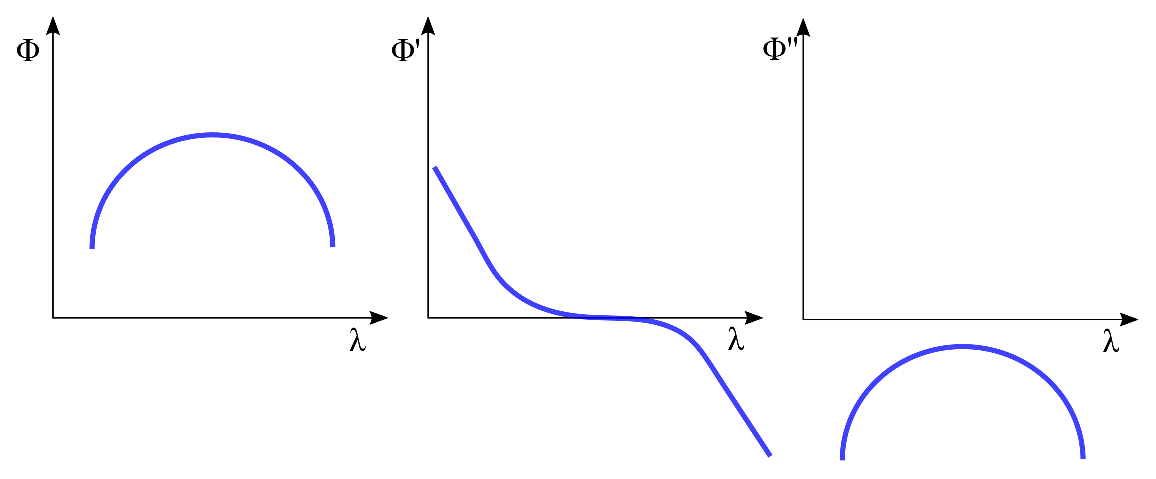
\includegraphics[width=\linewidth]{PhiConvex}
    \caption[Connection one to one between $\lambda$ and $a$]{Representation of the convex functional $\Phi[\lambda]$ and its first and second derivative.}
    \label{fig:PhiConvex}
\end{figure}
}


This argument is  valid for  any pair  of conjugate variables  and it
only depends on  the definition of the  conjugate variables introduced
in Eq. (\ref{relens1}).  It constitutes  the basic content of the DFT
when the relevant variable is the microscopic density operator.

Because the  connection is one  to one,  we may change  variables from
$\lambda$ to $a$.   However, the average $a$ is given  by a derivative
and such a  change of variables implies a loss  of information.  As we
know from the usual treatment in Thermodynamics \cite{Callen1960}, the
correct way to proceed is to  introduce the dimensionless entropy function $S[a]$ of
the given  level of description  as the (minus) Legendre  transform of
the thermodynamic potential in the form
\begin{align}
S[a] &=-\Phi[\lambda[a]]+\lambda[a] a
\label{entropya}\end{align}
The  relation of  this entropy  function $S[a]$  and the  Gibbs-Jaynes
entropy functional  ${\cal S}[\overline{\rho}]$ in  (\ref{entropy}) is
simple. The  former is just  the later  evaluated at its  maximum, the
relevant ensemble (\ref{relens1}). This is
\begin{align}
S[a]={\cal  S}[\overline{\rho}]
\end{align}
Because  the  entropy   $S[a]$  is  the  Legendre   transform  of  the
thermodynamic  potential  $\Phi[\lambda]$,  we have  the  relationship
conjugate to (\ref{cg1})
\begin{align}
  \frac{\partial S}{\partial a}&=\lambda
\label{e3}
\end{align}


\section{The dynamics}\label{Sec:Grabert}
In general it is possible to derive the evolution equation for a given
dynamic  variable  by  using  the technique  of  projection  operators
\cite{Kawasaki1973a,Grabert1982}. The projection operator method can be
understood, at its most fundamental level  as a way to approximate the
actual time dependent ensemble, which is the solution of the Liouville
equation, with a relevant  ensemble of the form (\ref{relens1}),
plus  a correction,  which  is the  responsible  for the  irreversible
behaviour. We  summarize   in  the   rest  of   this  section   the
time-dependent  projection  operator  technique as  presented  in  the
classical  textbook  by Grabert  \cite{Grabert1982}.   

The  aim is  to
derive equations of motion for  the time dependent average $a_i(t)$ of
the set of relevant variables $\hat{A}_i(z)$. The time dependent average
is
\begin{equation}
  a_i(t)={\rm Tr}[\rho_t\hat{A}_i]
  \label{ave}
\end{equation}
where $\rho_t$ is
the non-equilibrium solution of the Liouville equation. As it is shown
in  \cite{Grabert1982},  for  isolated systems  with a time-independent
Hamiltonian,  the   averages  (\ref{ave})  evolve  according   to  the
following closed exact equation

\begin{equation}
\frac{\partial }{\partial t} a_i(t)
= v_i(t) + \int_0^t dt' \sum_j K_{ij}(t,t') \lambda_j(t')
\label{ex}
\end{equation}
The reversible term is given by
\begin{equation}
v_i(t) = {\rm Tr}[\overline{\rho}_t  iL \hat{A}_i]
\label{vit}
\end{equation}
where $iL$ is the Liouville operator (\ref{iL}).

The  relevant
ensemble $\overline{\rho}_t$  is of  the form (\ref{relens1}),  with a
time   dependent  conjugate   variable  $\lambda(t)$.   The  conjugate
variables  $\lambda$ are  selected in  such  a way  that the  averages
$a(t)$ of the  real (i.e. the  solution of the Liouville equation) and of the relevant ensemble  coincide.  Note that
if   only  the   reversible  term   $v_i(t)$  would   be  present   in
Eq. (\ref{ex}), we would be  approximating the actual ensemble 
with a relevant  ensemble of
the form (\ref{relens1}), where the conjugate field $\lambda(t)$ is now
a function of time.  The error  in this approximation is, in fact, the
memory term which describes  irreversible behaviour.  The irreversible
term in Eq. (\ref{ex}) involves the memory kernel
\begin{equation}
K_{ij}(t,t') =
{\rm Tr}\left[\overline{\rho}_{t'} 
\left({\cal Q}_{t'} iL\hat{A}_j\right) G_{t't}
\left({\cal Q}_{t } iL\hat{A}_i\right)\right]
\label{ker}
\end{equation}
where   the  Kawasaki-Gunton   projection  operator   ${\cal  Q}_{t'}$
\cite{Kawasaki1973a,  Grabert1982}  applied  to an  arbitrary  function
$\hat{F}(z)$ is
\begin{eqnarray}
{\cal Q}_{t'}\hat{F}(z)& = &\hat{F}(z)- {\rm Tr}[\overline{\rho}_{t'} \hat{F}]
\nonumber\\
&-&\sum_i(\hat{A}_i(z)-a_i(t'))\frac{\partial }{\partial a_i(t')}
{\rm Tr}[\overline{\rho}_{t'} \hat{F}]
\label{Q}
\end{eqnarray}
Finally, the time ordered projected propagator $G_{t't}$ is given by formal series
\begin{eqnarray}
G_{t't}&=&1
+\sum_{n=1}^\infty \int_{t'}^tdt_1\cdots\int_{t'}^{t_{n-1}}dt_n
 iL{\cal Q}_{t_n}\cdots  iL{\cal Q}_{t_1}
\nonumber\\
&=&T_-\exp\left\{\int_{t'}^t dt''  iL{\cal Q}_{t''}\right\}
\end{eqnarray}
\Pendiente{where $T_-$ ensures that the operators are ordered from left to right as time increases.} \Note{¿Correcto?}
Eq.   (\ref{ex}) is  a closed  exact equation  for the  time dependent
averages $a(t)$.  The only assumption  taken in deriving (\ref{ex}) is
that the initial  ensemble to be used in the  Liouville equation is of
the relevant form.  This is, it is assumed that  the only knowledge at
the initial  time is the value  of the average $a(0)$  and, therefore,
the  least   biased  initial   ensemble  is   of  the   relevant  form
(\ref{relens1}).  Therefore, the time  dependent average $a(t)$ of the
relevant variables $\hat{A}(z)$  is computed with the  solution of the
Liouville equation $\rho_t(z)$  with an initial condition  which is of
the relevant  form.  The relevant  ensemble is a functional  of $a(t)$
through  $\lambda(t)$.   The kernel  becomes  a  functional of  $a(t)$
through the relevant  ensemble.  

Although Eq.  (\ref{ex})  is a closed
equation it is an integro-differential  equation which is difficult to
treat  in   general.   Nevertheless,  the  exact   transport  equation
(\ref{ex}) can  be approximated by  a memory-less equation  whenever a
clear separation  of time scales  exists between the evolution  of the
averages and  the decay of  the memory kernel. Under  this assumption
and the  neglect of terms of  order ${\cal O}( iL\hat{A}^3)$,  assumed to be
small due to  the slowness of the relevant variables,  one obtains the
Markovian equation \cite{Grabert1982}
\begin{equation}
\dot{a}_i(t) = v_i(t) + \sum_j D_{ij}(t) \lambda_j(t)
\label{ex2}
\end{equation}
where  the  dissipative matrix  is  given  by  the Green-Kubo  formula
\begin{equation}
D_{ij}(t)=\int_0^{\Delta t} dt'\left\langle 
{\cal Q}_t iL\hat{A}_j\exp\{iLt'\}{\cal Q}_t iL\hat{A}_i
\right\rangle^{\lambda(t)}
\label{dij}
\end{equation}
Here,  $\Delta t$ is  a  time large  compared  to the  decay  time of  the
correlation  integrand  but  short  in  front of  the  time  scale  of
evolution of  the relevant variables.  The  dissipative matrix depends
in general  on the  relevant variables  through the  relevant ensemble
and, as such, it is a function of time.  The dissipative matrix is, to
the  extent that  the  Markov property  holds,  positive definite  and
satisfies Onsager's reciprocity \cite{Grabert1982}. 

It is straightforward  to show that the  dynamic equations (\ref{ex2})
have  as  a  Lyapunov   function  the  entropy  (\ref{entropya})  and,
therefore,   the   dynamics   complies   with  the   Second   Law   of
Thermodynamics.  The  equations (\ref{ex2})  predict the decay  of any
initial value  of the  average of the  relevant variables  towards its
unique equilibrium  values. Forced situations may  be treated
with the present  formalism \cite{Grabert1982} but we  do not consider
them here for simplicity.





\section{Summary}

In this chapter we have introduced two important concepts that holds this dissertation. The first one, quasi-equilibrium, states that what we refer to equilibrium of a system depends on the time window we take. If the time of obervation is shorter than the time in which some variables evolve, we may use this variables as CG variables. Because the other variables evolve faster we may assume that are irrelevant for the selected level of description. Therefore, we say that the slow and faster variables evolve in different time scales, which is the second important concept of this chapter. Only when there is a well-separation of time scales we obtain tractable time evolution equation without memory terms. This is known as Markovian descripcion to distinguish from the non-Markovian description in which the present state is determined by the past. 

Under the Markovian aproximation, we obtain the general form of the memory-less dynamic equation of the selected variables. In the next chapter we will use this equation to obtain the dynamic equations of the CG variables of a system consisting on a liquid between two solid slabs.  

%We have introduced the relevant ensemble, $\bar{rho}$, based on the idea that the least biased probability distribution function is the one which maximazes the Shannon's entropy functional, which evaluated at its maximum (i.e. the relevant ensemble) is equal to the entropy function $S[a]$ obtained as the legendre transform of the thermodynamic potential $\Phi[\lambda]$.


%-----------------------------------------------------------------
%CHAPTER 2
%-----------------------------------------------------------------
\chapter{Nanoscale hydrodynamics near solids}\label{Chap:Theory}
\markboth{Nanoscale hydrodynamics near solids}{}
\epigraph{\textit{There is no future. There is no past. Do you see? Time is simultaneous, an intricately structured jewel that humans insist on viewing one edge at a time, when the whole design is visible in every facet.}}{Watchmen \\ ALAN MOORE} 
%No hay futuro. No hay pasado ¿Lo ves? El tiempo es simultáneo, una joya de una estructurada demasiado compleja en donde los humanos se empeñan en solo ver un borde, cuando el diseño por completo es visible en todas las facetas.-Alan Moore.
In this chapter 
\includepdf[page=-]{00-Second-Submission26dic2017.pdf}

\chapter{A solution to the plateau problem in the Green-Kubo formula}\label{Chap:GKcorrected}
\markboth{A solution to the plateau problem in the Green-Kubo formula}{}
\epigraph{\textit{Falta cita.}}{Título \\ AUTOR}
In this chapter
\includepdf[page=-]{2nd-sub-GK-corrected.pdf}

\chapter{Theory for planar flows with confinig walls}\label{Chap:Planar}
\markboth{Theory for planar flows}{}
\epigraph{\textit{Nothing got inside the head without becoming pictures.}}{The corrections \\ JONATHAN FRANZEN}
\includepdf[page=-]{003-Planar-Theory-27dic2018.pdf}

\chapter{Space and time locality for unconfined fluids}\label{Chap: PBC}
\markboth{Space and time locality for unconfined fluids}{}
\epigraph{\textit{Time is longer than any distance.}}{Absalom, Absalom! \\ WILLIAM FAULKNER}
\includepdf[page=-]{005-Mori-PBC-10oct2018.pdf}

\chapter{Non-Markovian behaviour near solids walls}\label{Chap:Walls}
\markboth{Markovian behaviour near solids}{}
\epigraph{\textit{Descubrir es ver de otro modo lo que nadie ha percibido.}}{Blanco Nocturno \\ RICARDO PLIGIA}
\includepdf[page=-]{006-Mori-Correlations-Walls.pdf}


\chapter{The slip boundary condition}
\label{Chap:Slip}
\markboth{The slip boundary condition from MD simulations}{}
\epigraph{\textit{It is remarkable how long men will believe in the bottomlessness of a pond without taking the trouble to sound it.}}{Walden \\ HENRY DAVID THOREAU}
\includepdf[page=-]{007-BC-Simulations.pdf}

\chapter{Conclusions}\label{Chap:Conclusions}
\epigraph{\textit{The runner runs truly to the end.}}{Once a runner \\ JOHN L. PARKER}




\bibliographystyle{unsrt}
\bibliography{../bibTex/thesis-library}

%---------
% APPENDIX
%---------
\pagestyle{noHeader}
\begin{appendices}
%\appendix
\chapter{Contributions}\label{Ap:Contributions}
The following published articles and posters are related with this dissertation.
\begin{enumerate}
  \item Nanoscale hydrodynamics near solids.
  \item Discrete hydrodynamics near solids for planar flows.
  \item Revisiting the plateau problem in the Green-Kubo formula.
  \item Space and time locality of discrete hydrodynamics.
  \item Non-Markovian behaviour of discrete hydrodynamics near solids.
  \item The slip boundary condition from MD simulations revisited.
  \item Fises Sevilla
  \item Ucrania
  \item IWNET
  \item Fises Madrid
\end{enumerate}

\chapter{List of Acronyms}\label{Ap:Acronyms}
\begin{tabular}{l l}
    CM   & Classical Mechanics \\
    DFT  & Density Functional Theory \\
    DDFT & Dynamic Density Functional Theory \\
    GLE  & Generalized Langevin Equation \\
    LADM & Local Average Density Model \\
    LJ   & Lennard-Jones \\
    LFSA & Linear For Spiky Approximation \\
    MD   & Molecular Dynamics \\
    NEMD & Non-Equilibrium Molecular Dynamics\\
    NESM & Non-Eauilibrium Statistical Mechanics \\
    QM   & Quantum Mechanics \\
    SM   & Statistical Mechanics \\
    ToCG & Theory of Coarse-Graining \\
\end{tabular}


\chapter{Physical parameters and variables}
\begin{tabular}{l l}
    $m$ & mass particles \\
    $L_x, L_y, L_Z$ & dimensions of the simulations box \\
    $M'$ & mass solid sphere \\
    $M$ & mass solid walls \\
    $N$ & Number of liquid particles \\
    $N'$ & Number of solid particles \\
    $N_{\rm bins}$ & Number of bins \\
    $k_B$ & Boltzmann's constant \\
    $T$ & Temperature \\
    $\beta$ & $(k_BT)^{-1}$ \\
    $\Delta z$ & distance between two nodal planes \\
    $\delta_{\mu\nu}$ & Kronecker delta \\
    ${\cal F}[]$ & Free energy functional \\
    $F()$ & Free energy function \\
\end{tabular}
\end{appendices}

\end{document}
